% This syllabus template was created by:
% Brian R. Hall
% Associate Professor, Champlain College
% www.brianrhall.net

% Document settings
\documentclass[11pt]{article}
\usepackage[margin=1in]{geometry}
\usepackage[pdftex]{graphicx}
\usepackage{multirow}
\usepackage{setspace}
\pagestyle{plain}
\setlength\parindent{0pt}

\begin{document}

% Header
\begin{tabular}{ c | c | c | c }
{
\includegraphics[height=0.75in,width=1.25in]{latex.png}} & 
{
\includegraphics[height=0.75in,width=1.25in]{markdown.png}} &
{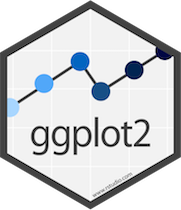
\includegraphics[height=0.75in,width=0.75in]{ggplot2.png}} &
{
\includegraphics[height=0.75in,width= 0.75in]{github.png}} 
\end{tabular} 
\\\\

% Course information
\begin{tabular}{ l l }
  & \LARGE Coding for Visualization in Ecology (Ecol 592) \\
\end{tabular}
\vspace{10mm}

% Teacher information
\begin{tabular}{ l l l l } % These are Ls for left alignment btw, not vertical slash..
  & \large Ava Hoffman & Clif McKee & Very distinguished Prof. \\
  Contact: & \footnotesize avamariehoffman@gmail.com & \footnotesize clifton.mckee@gmail.com & \footnotesize email\\
  Office:  & BIO 339 & & \\
  Office Hours: & by appointment & &
  \end{tabular}
\vspace{5mm}
\begin{center}   \LARGE Course website: github.com/avahoffman/course.url... \\
\end{center}

% Course details
\textbf {\large Course Description:} Careers using programming are growing fast, about 50\% faster than other jobs [1]. This course aims to familiarize ecology students with several key programming languages/packages that will benefit them in graduate school and in their future careers. With a focus on visualization, students will take a goal-based approach to learning. After a brief introduction to the language or package, students will work on tangible products including:
\begin{itemize}
\item a resume or CV using \LaTeX
\item a project summary/outline using Markdown
\item figure(s) using the student's own data in the R package ggplot
\item a publicly visible code repository on GitHub using command line
\end{itemize}
Students will work in several-hour long chunks to cultivate a workshop-like environment conducive to questions and student teaching.\\\\
\textbf {\large Prerequisites:} Some familiarity with R or SAS; some data/project basis to work with; curiosity.\\\\
\textbf {\large Credit Hours:} 1 \\

\textbf {\large Course Objectives:} \\
At the completion of this course, students will be able to demonstrate a tangible product based on their new coding knowledge.\\

% I recommend using \newpage here if necessary
\textbf {\large Grade Distribution:} \\
Based on final product produced and class attendance. Because sessions are long and limited in number, alternative assignments may be assigned for students who have to miss a session (eg., explore Shiny/knitr).

% A new page is forced here.
\newpage

% Course Outline
\textbf {\large Tentative Course Outline}:

\begin{table}[h!]
\normalsize % The size of the table text can be changed depending on content. Remove if desired.
\begin{tabular}{ | c | c | }
\hline
\textbf{Week} & \textbf{Content} \\
\hline
Week 1 & \begin{minipage}{.85\textwidth}
\begin{itemize} \itemsep-0.4em
	\vspace{1mm}
	\item Something interesting
	\item Reading assignment: Something interesting
	\vspace{1mm}
\end{itemize}
\end{minipage} \\
\hline
Week 2 & \begin{minipage}{.85\textwidth}
\begin{itemize} \itemsep-0.4em
	\vspace{1mm}
	\item Something interesting
	\item Reading assignment: Something interesting
	\vspace{1mm}
\end{itemize}
\end{minipage} \\
\hline
Week 3 & \begin{minipage}{.85\textwidth}
\begin{itemize} \itemsep-0.4em
	\vspace{1mm}
	\item Something interesting
	\item Reading assignment: Something interesting
	\vspace{1mm}
\end{itemize}
\end{minipage} \\
\hline
Week 4 & \begin{minipage}{.85\textwidth}
\begin{itemize} \itemsep-0.4em
	\vspace{1mm}
	\item Something interesting
	\item Reading assignment: Something interesting
	\vspace{1mm}
\end{itemize}
\end{minipage} \\
\hline
\end{tabular} 
\end{table}

[1] https://www.burning-glass.com/research-project/coding-skills/
\end{document}

